%%%%%%%%%%%%%%%%%%%%%%%%%%%%%%%%%%%%%%%%%
% Developer CV
% LaTeX Template
% Version 1.0 (2019-11-25)
%
% This template originates from:
% http://www.LaTeXTemplates.com
%
% Authors:
% Mikhail f. Shiryaev (mikhail.f.shiryaev@gmail.com)
% Based on template by Jan Vorisek (jan@vorisek.me)
% Based on a template by Jan Küster (info@jankuester.com)
% Modified for LaTeX Templates by Vel (vel@LaTeXTemplates.com)
%
% License:
% The MIT License (see included LICENSE file)
%
%%%%%%%%%%%%%%%%%%%%%%%%%%%%%%%%%%%%%%%%%

%----------------------------------------------------------------------------------------
%  PACKAGES AND OTHER DOCUMENT CONFIGURATIONS
%----------------------------------------------------------------------------------------

\documentclass[11pt]{developercv} % Default font size, values from 8-12pt are recommended
\usepackage{xstring}
\usepackage{graphicx}

\StrSubstitute{\jobname}{^^^^0022}{}[\Title] % ^^^^0022 is a double quote to avoid linter warning

\title{\Title}


\hypersetup{pdftitle=Alexandra Shiryaeva -- \Title,  % chktex 8
  pdfauthor=Alexandra Shiryaeva,
  colorlinks=true,
  linkcolor=blue,
  urlcolor=darkgray,
}

%----------------------------------------------------------------------------------------

\begin{document}

%----------------------------------------------------------------------------------------
%  TITLE AND CONTACT INFORMATION
%----------------------------------------------------------------------------------------

\begin{minipage}[t]{0.39\textwidth} % 45% of the page width for name
  \vspace{-\baselineskip} % Required for vertically aligning minipages
  \colorbox{black}{{\huge\textcolor{white}{\textbf{\MakeUppercase{Alexandra}}}}} % First name

  \colorbox{black}{{\huge\textcolor{white}{\textbf{\MakeUppercase{Shiryaeva}}}}} % Last name
  \colorbox{black}{{\LARGE\textcolor{white}{\textbf{Geo-Daten Analyst}}}} % Last name

  \hyphenpenalty=10000
  \raggedright{}
  %{\huge \Title} % Career or current job title
\end{minipage}
\begin{minipage}[t]{0.45\textwidth} % 27.5% of the page width for the first row of icons
  \vspace{-\baselineskip} % Required for vertically aligning minipages
  \icon{MapMarker}{18}{Hamburg DE}\\
  \icon{Phone}{18}{+49 177 6460919}\\
  \icon{At}{18}{\href{mailto:alexandra.v.shiryaeva@gmail.com}{alexandra.v.shiryaeva@gmail.com}}\\
\end{minipage}
\begin{minipage}[t]{0.35\textwidth} % 27.5% of the page width for the second row of icons
  \vspace{-\baselineskip} % Required for vertically aligning minipages
  % The first parameter is the FontAwesome icon name, the second is the box size and the third is the text
  % Other icons can be found by referring to https://ctan.net/fonts/fontawesome/doc/fontawesome.pdf and using the word after \fa in the command for the icon you want
  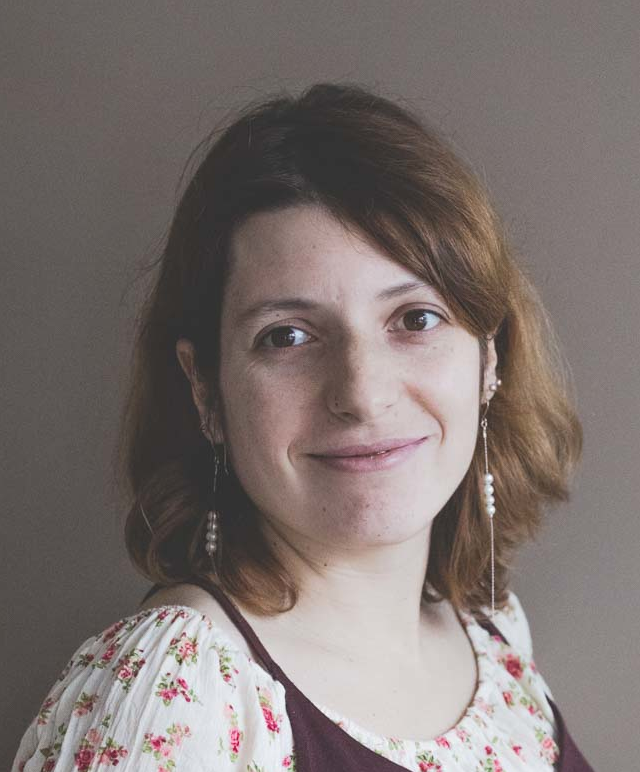
\includegraphics[scale=0.13]{Photo.png}
\end{minipage}

\vspace{0.2cm}

%----------------------------------------------------------------------------------------
%  Personal data
%----------------------------------------------------------------------------------------

\cvsect{Persönliche Daten}

{\large{Geboren am 14.12.1985 in Schukowski, Moskau, Russland\\
Staatsangehörigkeit – russisch\\
Aufenthaltserlaubnis in Deutschland, Erwerbstätigkeit gestattet}}
\\\\

%----------------------------------------------------------------------------------------
%  EXPERIENCE
%----------------------------------------------------------------------------------------

\cvsect{Berufserfahrung}

\begin{entrylist}
  \entry{2010 --- now*}
    {Wissenschaftliche Mitarbeiterin\\}
    {Klimalabor, Institut für Geographie der Russischen Akademie der Wissenschaften}
    {\
      • Arbeit mit großen Mengen meteorologischer Daten (mit Excel, MySQL, Python): Qualitätskontrolle, statistische Analyse, Datenvorbereitung für die Visualisierung\\
      • Erstellen von Karten in GIS (Surfer, QGIS, ArcGIS), Schreiben von Skripten für die Datenvisualisierung in Python mit numpy und maplotlib)\\
      • Datenanalyse und Verfassung wissenschaftlicher Publikationen zum Klimawandel in russischer und englischer Sprache (12 Artikel in Fachzeitschriften)\\
      • Durchführung meteorologischer Beobachtungen bei Feldexpeditionen (Nordrussland, Kaukasus, Spitzbergen)\\
      • Vorträge bei wissenschaftlichen Konferenzen\\\\
      {\footnotesize* 04/2010 – 09/2017 Vollzeittätigkeit, seit 10/2017 Teilzeittätigkeit (Homeofice aus Deutschland)}
    }
  \entry{2008 --- 2015\\(Teilzeittätigkeit)}
    {Expertin in der Abteilung Marketing und Entwicklung\\}
    {Roshydromet (Bundesdienst für Hydrometeorologie und Umweltmonitoring Russlands)}
    {\
      • Untersuchungen zur Verwertung nach Wetterinformationen in der Wirtschaft\\
      • Erstellung von Analysen, Berichten und Präsentationen\\
      • Vorbereitung von Werbematerialien\\
      • Bearbeitung der Kundenfragebogen\\
      • Meteorologische Unterstützung der Olympischen Winterspiele 2014 in Sotschi (Organisation von Weiterbildungen und Tagungen für Meteorolog*innen, Vorbereitung von Schulungsunterlagen)\\
    }
\end{entrylist}


%----------------------------------------------------------------------------------------
%  EDUCATION
%----------------------------------------------------------------------------------------

\cvsect{Bildungsweg}

\begin{entrylist}
  \entry{2007 --- 2009}
    {Master in Meteorologie und Klimatologie\\}
    {Staatliche Lomonossow-Universität Moskau, Fakultät für Geographie}
    {Masterarbeit ``Veränderungen von wirtschaftlich relevanten klimatologischen Parametern in der kalten Jahreszeit in Russland im Zeitraum 1950–2006''}
  \entry{2003 --- 2007}
    {Bachelor in Meteorologie und Klimatologie\\}
    {Staatliche Lomonossow-Universität Moskau, Fakultät für Geographie}
    {Bachelorarbeit ``Veränderung der Schneehöhe und Intensität von Schneefällen und deren Auswirkungen auf die Straßenreinigungskosten in russischen Städten''}
\end{entrylist}

\cvsect{Weiterbildung}
\begin{entrylist}
  \shortentry{04/2020-06/2020}{Sprachkurs Deutsch B1 Sprachschule ``DeutschOnline''}
  \shortentry{11/2018-12/2018}{Sprachkurs Deutsch A2 University Service, Hamburg}
  \shortentry{02/2018-04/2018}{Sprachkurs Deutsch A1.2-A2.1 DeutschAkademie, Hamburg}
  \shortentry{01/2012-01/2012}{European Research Course of Atmospheres Grenoble, France}
\end{entrylist}

%----------------------------------------------------------------------------------------
%  ADDITIONAL INFORMATION
%----------------------------------------------------------------------------------------

\cvsect{IT-Kenntnisse}

  Betriebssystem: Windows, Linux\\
  MS Office: Word, Excel, Power Point --- sehr gute Kenntnisse\\
  Grafikprogramme: Adobe Photoshop, GIMP --- gute Kenntnisse\\
  GIS:\@ Surfer --- sehr gute Kenntnisse; ArcGIS, QGIS --- gute Kenntnisse\\
  SQL, Python --- Grundkenntnisse\\

\cvsect{Sprachen}

Russisch Muttersprache\\
Deutsch gute Kenntnisse\\
Englisch sehr gute Kenntnisse\\

\cvsect{Interessen}

Reisen, Wandern, Joggen

%----------------------------------------------------------------------------------------

\end{document}
